\documentclass[10pt]{beamer}

\usetheme[
%%% options passed to the outer theme
%    hidetitle,           % hide the (short) title in the sidebar
%    hideauthor,          % hide the (short) author in the sidebar
%    hideinstitute,       % hide the (short) institute in the bottom of the sidebar
%    shownavsym,          % show the navigation symbols
%    width=2cm,           % width of the sidebar (default is 2 cm)
%    hideothersubsections,% hide all subsections but the subsections in the current section
%    hideallsubsections,  % hide all subsections
    left               % right of left position of sidebar (default is right)
%%% options passed to the color theme
%    lightheaderbg,       % use a light header background
  ]{AAUsidebar}

% If you want to change the colors of the various elements in the theme, edit and uncomment the following lines
% Change the bar and sidebar colors:
%\setbeamercolor{AAUsidebar}{fg=red!20,bg=red}
%\setbeamercolor{sidebar}{bg=red!20}
% Change the color of the structural elements:
%\setbeamercolor{structure}{fg=red}
% Change the frame title text color:
%\setbeamercolor{frametitle}{fg=blue}
% Change the normal text color background:
%\setbeamercolor{normal text}{bg=gray!10}
% ... and you can of course change a lot more - see the beamer user manual.


\usepackage[utf8]{inputenc}
\usepackage{comment}
\usepackage{lmodern}
\usepackage{ucs}
\usepackage{t1enc}
\usepackage[english]{babel}
%\usepackage[T1]{fontenc}
% Or whatever. Note that the encoding and the font should match. If T1
% does not look nice, try deleting the line with the fontenc.
\usepackage{helvet}

\usepackage{subcaption}
\captionsetup{compatibility=false}

% colored hyperlinks
\newcommand{\chref}[2]{%
  \href{#1}{{\usebeamercolor[bg]{AAUsidebar}#2}}%
}


\date{}


	\title{PsyLog: Søvn og Aktivitetsmoduler for Personer med Affektive Lidelser}
	\author[sw808f15]{
			Lasse Vang Gravesen \\
			Søren Skibsted Als\\
			Lars Andersen \\
			Mathias Winde Pedersen
}
	
% - Give the names in the same order as they appear in the paper.
% - Use the \inst{?} command only if the authors have different
%   affiliation. See the beamer manual for an example




% specify a logo on the titlepage (you can specify additional logos an include them in 
% institute command below
\pgfdeclareimage[height=1.5cm]{titlepagelogo}{AAUgraphics/aau_logo_new} % placed on the title page
%\pgfdeclareimage[height=1.5cm]{titlepagelogo2}{graphics/aau_logo_new} % placed on the title page
\titlegraphic{% is placed on the bottom of the title page
  \pgfuseimage{titlepagelogo}
%  \hspace{1cm}\pgfuseimage{titlepagelogo2}
}

\graphicspath{ {Media/} }
\newcommand{\btVFill}{\vskip0pt plus 1filll}

\begin{document}
% the titlepage
{\aauwavesbg%
\begin{frame}[plain,noframenumbering] % the plain option removes the sidebar and header from the title page
  \titlepage
\end{frame}}
		
\section{Introduktion}

\begin{frame}
\frametitle{Samarbejde}

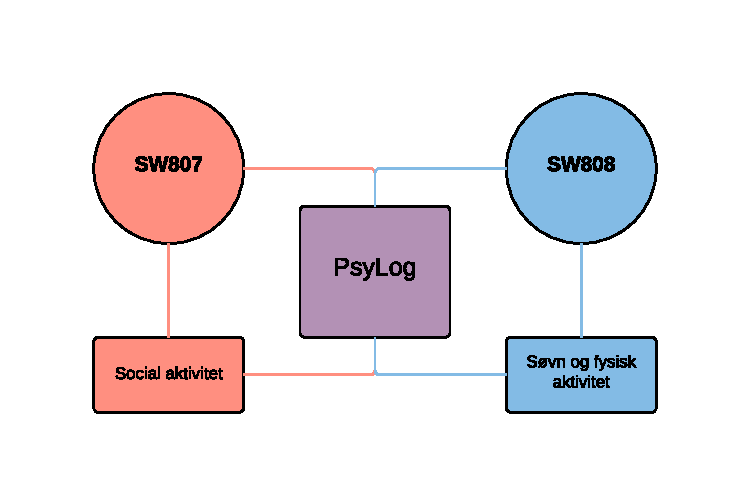
\includegraphics[width=\textwidth]{graphics/samarbejde.pdf}

\end{frame}

\subsection{Nuværende situation}

\begin{frame}
\frametitle{Diagnostisering}

\begin{itemize}
\item Egen læge, viderestillet
\item Indlæggelse ved slemmere tilfælde
\item Opfølgende møder
\item Interview til vurdering
\end{itemize}

\end{frame}

\begin{frame}
\frametitle{Problemer}
\begin{itemize}
\item Forværring opdages for sent
\item Kræver meget kontakt med behandler
\item Kun lav-frekvens indsamling/vurdering
\item Subjektive besvarelser, afhænger af patienten
\item xx Familie/venners vurdering, ud fra observation af adfærd
\item Egen observation og selvhjælp
\end{itemize}

\end{frame}

\begin{frame}
\frametitle{Forbedring via software}

\begin{itemize}
\item Kontinuert indsamling af data vedrørende adfærd
\item Indsamling af data mellem møder med behandler
\item Støtte selvhjælp bedre
\item Mere objektiv data
\end{itemize}

\end{frame}

\section{Affektive Lidelser}

\begin{frame}
\frametitle{Definition}

\end{frame}

\begin{frame}
\frametitle{Stemningsleje}

\end{frame}

\section{Brochure med idéer}

\begin{frame}
\frametitle{Formål med brochure}

\begin{itemize}
\item Indledende undersøgelse
\item Muligheder for dataindsamling
\item Knytning mellem (analyseret) data og symptomer
\item Udgangspunkt til diskussion med eksperter
\end{itemize}

\end{frame}

\section{Platform}

\begin{frame}
\frametitle{Kriterier}
Baseret på metaforen "f-16 fly"
\begin{itemize}
\item Modulær
\item Fleksibel
\item Kombinerbar
\item Kommunikativ
\end{itemize}
\end{frame}

\begin{frame}
\frametitle{Arkitektur}
\begin{figure}[h]
	\centering						%  l   b   r	t
	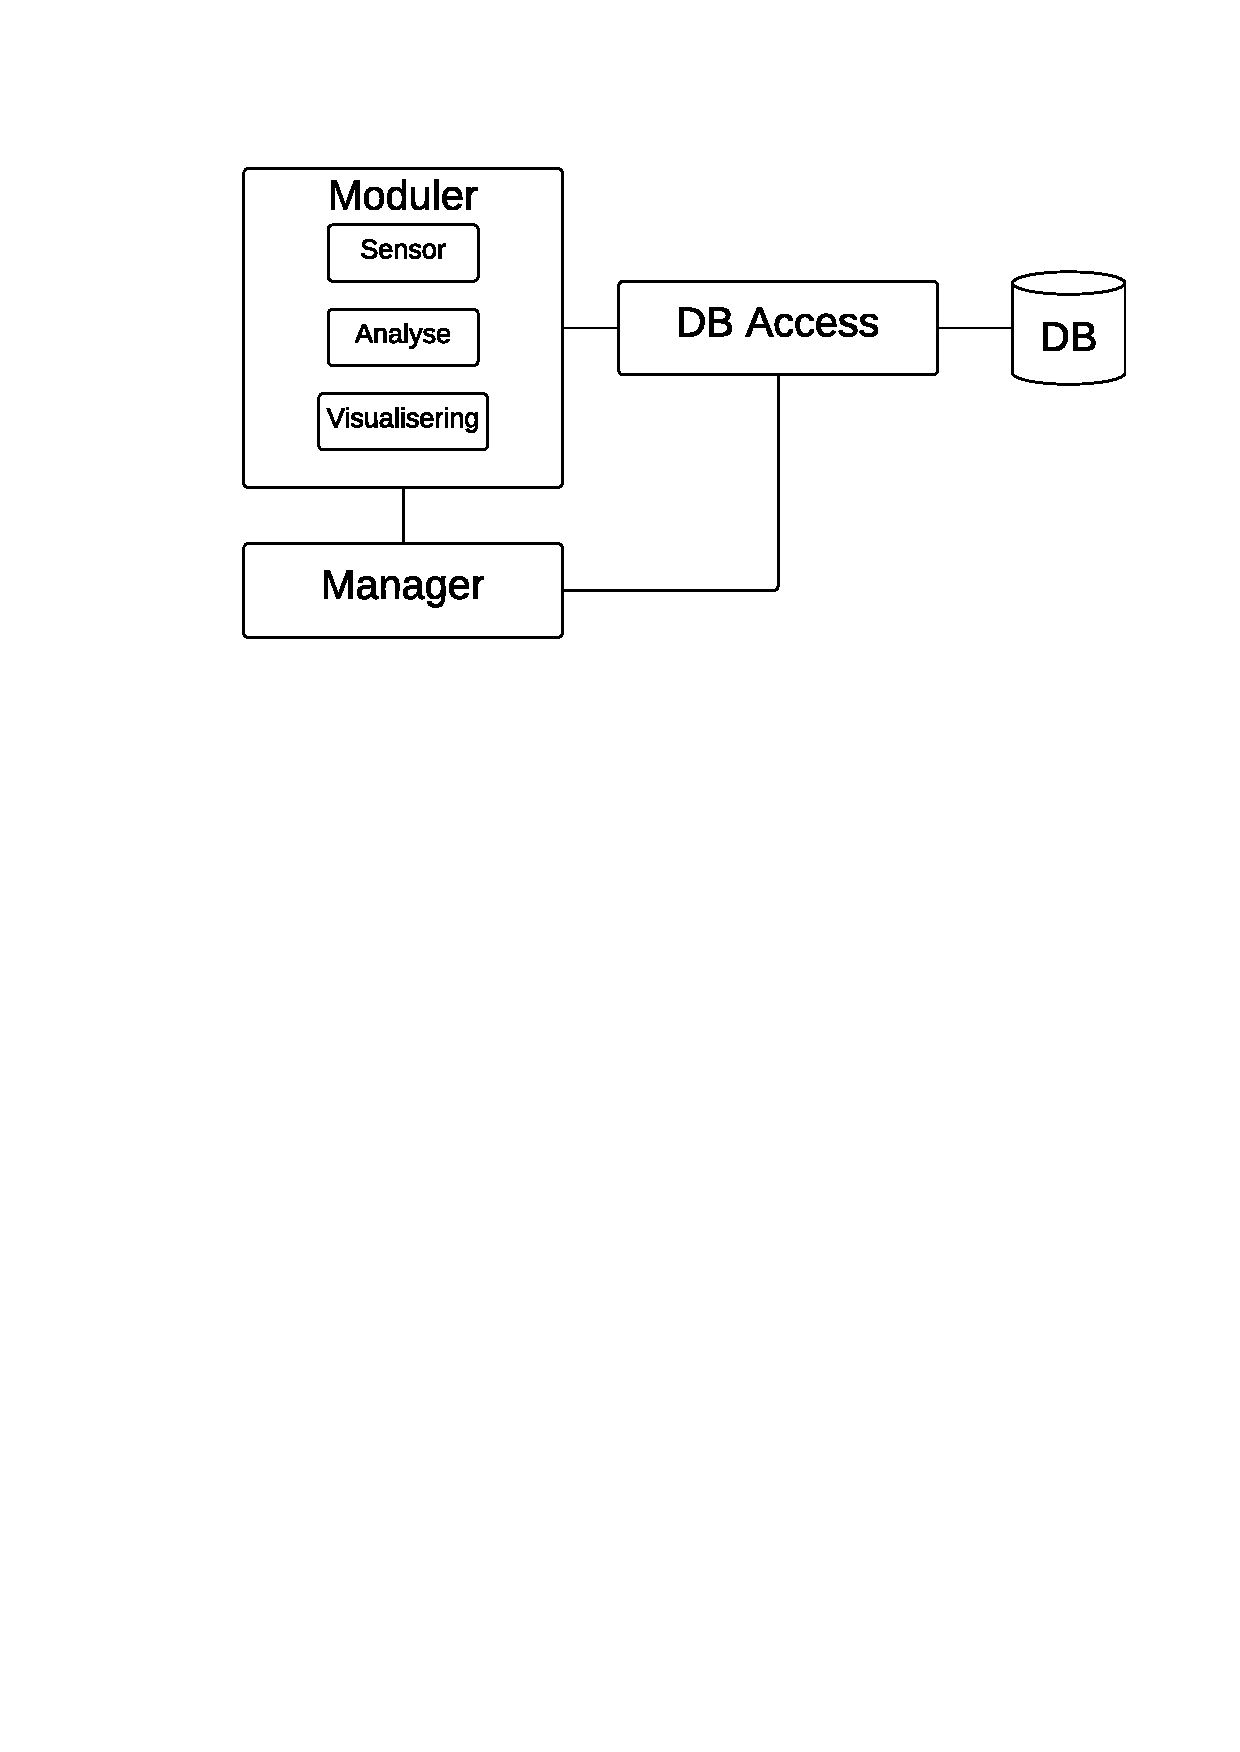
\includegraphics[scale=0.5, trim = 1cm 17.5cm 1cm 1cm, clip]{graphics/ArkitekturLucidChart}
	\caption{Systemets arkitektur}
  \label{arkitektur_udkast_1}
\end{figure}
\end{frame}

\begin{frame}
\frametitle{arkitektur - DB}
\begin{itemize}
\item Data fra alle moduler
\end{itemize}
\end{frame}

\begin{frame}
\frametitle{arkitektur - DB Access}
\begin{itemize}
\item Adgangslag til DB
\item Muliggør abstraktion over data lokation
\end{itemize}
\end{frame}

\begin{frame}
\frametitle{arkitektur - Moduler}
\begin{itemize}
\item 3 typer
\begin{itemize}
\item Data
\item Analyse
\item Visning
\end{itemize}
\item Hver kan bruge data fra de andre
\end{itemize}
\end{frame}

\begin{frame}
\frametitle{arkitektur - Manager}
\begin{itemize}
\item Central kontrol enhed
\item Del brugeren interagerer med
\item Kontrollerer hvilke moduler der skal køre 
\end{itemize}
\end{frame}

\begin{frame}
\frametitle{Arkitektur - Kriterier}
Kriterierne dækkes af følgende elementer i arkitekturen:
\begin{itemize}
\item Modulær -> Moduler
\item Fleksibel -> Manager
\item Kombiner -> Moduler
\item Kommunikativ -> DB Access/DB
\end{itemize}
\end{frame}

\begin{frame}
\frametitle{Eksempel}
\begin{itemize}
\item Krav til start på modul navn
\begin{itemize}
\item dk.cs.aau.psylog.sensor
\item dk.cs.aau.psylog.analysis
\item dk.cs.aau.psylog.view
\end{itemize}
\item Valid JSON-skema(Bilag D)
\end{itemize}
\end{frame}


I udviklingsforløbet af platformen, var der forskellige beslutninger, som blev taget i henhold til hvad der skulle implementeres, samt hvad der kunne udvikles videre på og generelle overvejelser om platformen.
At reflektere over disse beslutninger og overvejelser skaber overblik og forståelse af forløbet, og er beskrevet herefter.

%\section{Valg af data kilder}
%Hvilke data kilder man bruger i for eksempelvis et analyse modul kan være vigtige, idet hvis man for eksempel har data fra et smartwatch og fra en accelerometer på smartphonen og en af disse viser ingen bevægelse ville det være en god idé at hvis modulet selv kunne evaluere hvilke kilde den skal tage data fra. 
%Men dette blev aldrig lavet, idet det ikke var tænkt særlig vigtigt og at ressourcerne var begrænsede og skulle bruges på andre opgaver i stedet for.

\section{Kontekst}
Konteksten for brugen af applikationen er ikke blevet arbejdet med.
Man kunne forstille sig at der kunne være indbyggede moduler til at registrere hvilket kontekst smartphonen befinder sig i.
Dette kunne være at finde ud af om smartphonen befinder sig på en person eller om den er i en jakkelommer, på et natbord eller lignende.
Hvis det er muligt at identificere konteksten, kan det være yderst brugbar information for analysemoduler, til at hjælpe dem med at afgøre hvordan forskellige former for data skal behandles.
Her kunne man for eksempel forestille sig at lyd var yderst relevant hvis enheden var på en person, men irrelevant hvis den lå i en jakkelomme.
Der er også den mulighed at platformen ud fra konteksten vælger hvilke datakilder, der stadig er relevante at se på, men en sådan måde at beslutte på vil reducere platformens modularitet, så det vil være bedre at overlade det til det enkelte modul at beslutte hvad der er relevant for den givne kontekst.

Dog vides det ikke om en sådan klassificering kan opnå den fornødne præcision, men undersøgelse af det vil bestemt være værd at overveje.

\section{Brugerinteraktion}
En række refleksioner går på brugerinteraktion.
Dette inkluderer refleksion af visualiseringer, interaktive moduler, notifikationer og huskekort, hvilket er beskrevet herunder.

\subsection{Visualiseringer}
Data indsamlet og analyseret af forskellige moduler, skulle originalt kunne visualiseres, med det formål at give brugere af platformen et overblik over deres sindstilstand.
I \cref{modul_definition}, blev der diskuteret hvordan håndteringen af visualiserings-modulerne skal foretages.
Dette er et emne, der bør udforskes ved videre arbejde, men er ikke foretaget på nuværende tidspunkt, da det blev dømt for tidskrævende.
Ved videre arbejde bør datavisualiserings-teknikker og -teori undersøges nærmere.

\subsubsection{Hvordan skal brugeren vælge visualiserings moduler?}
Udover diskussion om hvilke krav der skal være til visualiserings-moduler, beskrevet i \cref{modul_definition}, skal man også overveje hvordan brugere skal vælge hvilke visualiserings-moduler de gerne vil kunne se, og hvordan de skal vises i manageren.

En mulighed er at have en administrationsside til visualiseringer, der minder om indstillingssiden til valg af dataindsamlings- og analysemoduler.
Eksempelvis kan man forestille sig en kobling mellem disse moduler og visualiseringerne, sådan at for hvert modul kan man angive hvilke visualiseringer man vil benytte.
Koblingen ville her gå på visualiseringer, der passer til de enkelte datasæt som modulerne tilbyder.

En anden mulighed er at visualiserings-modulerne, der er installeret, er dem der bliver vist i manageren, og specificerer selv hvilke moduler de virker til.
Dette er en mere enkel løsning at implementere, til gengæld tilbyder den knap så stor fleksibilitet i forhold til udviklingen af nye analysemoduler, da man så er nødsaget til at skulle opdatere specifikationen for de pågældende visualiserings-moduler.

\subsubsection{Hvordan skal visualiseringer vises i manageren?}
En anden diskussion går på hvorledes visualiseringerne skal vises i manageren.
En enkel måde at gøre dette på er som en liste, der bliver præsenteret på forsiden af manageren.
Der vil med denne løsning være mulighed for at ændre rækkefølgen af modulerne ved at trække visualiseringerne til en anden position i listen.
En ulempe ved denne løsning er at den ikke tilbyder kategorisering af visualiseringer.

En inddeling af visualiseringerne i forskellige kategorier ved hjælp af faner er et alternativ, der kan benyttes.
Dette sikrer at hvis man har mange visualiseringer bliver det nemmere at abstrahere over disse, da man kan nøjes med at se på en kategori ad gangen, eksempelvis søvn eller social aktivitet.

\subsubsection{Hvordan skal visualiseringer gøres forståelige?}
Endvidere er der en overvejelse, som går på at udvikle visualiseringer, der er forståelige og gennemskuelige for målgruppen, men dette betragtes som et ansvar for den enkelte visualiserings-udvikler og er dermed ikke noget platformen bør takle.
Platformen benyttes af udvikleren, men hvordan de enkelte visualiseringer skal se ud er op til den enkelte udvikler.

De præsenterede muligheder er ikke fastlagte, og opfordres til at blive diskuteret yderligere ved videre arbejde, så den mest hensigtsmæssige løsning opnås.

\subsection{Interaktive moduler}
En idé, som ikke blev undersøgt var at udvikle interaktive moduler.
Eksempelvis kunne patienter blive sat til at løse matematiske problemer for at teste deres kognitive evner eller spille `balance the ball' for at teste deres reaktionsevne.
Dette kunne være en god idé, da man ved affektive lidelser nogle gange ser den slags symptomer, for eksempel ved depression kan man tit opleve at man har svært ved at huske detaljer, tage beslutninger eller koncentrere sig og hvis spil kunne laves for at teste disse kunne man få et indblik i hvordan patienterne har det. 
En yderlig grund til at undersøge og implementere dette er, at det vil gøre systemet mere interessant for brugerne og give dem en grund til at bruge det hver dag. 
Et sådant modul ville klassificeres som en mellemting mellem et visualiserings modul og et sensor modul.
Visualisering da modulet skal vise noget til brugeren og sensor da den giver data, der kan bruges af analysemoduler til at få et indblik i folks tilstand.

\subsection{Notifikationer}
Noget, som også blev diskuteret tidligere i projektforløbet var at give notifikationer til brugeren, herunder det, som tidligere er benævnt som interventioner.
Dette blev dog tilsidesat, da det blev vurderet at der var for mange faldgruber i.f.t. at forstyrre en evt. patient med psykiske problemer.
Dog erfarede vi senere, i forbindelse med styregruppemødet, at patienterne er meget interesseret i at få at vide så tidligt som muligt om de er under forværring i deres tilstand.

Der kunne eksempelvis gives to slags informationer; interventionen, som direkte siger at der foregår en forværring eller at der har været en drastisk stigning/fald i.f.t. sensor/analyse.
Den anden slags information kan være noget opsummerende og mere neutralt, så der ikke på samme måde skal evalueres om hvorvidt der er ved at ske en forværring, derimod blot præsentere noget af det seneste data fra en sensor/analyse.
Det andet eksempel på en notifikation kunne få brugeren til at reflektere over sin situation, hvis der for eksempel kunne ses et tydeligt fald i søvnkvalitet eller antal sociale interaktioner, men uden direkte at sige noget om en evt. forværring.

\subsubsection{Huskekort}
I interviewet med psykolog Janne Vedel Rasmussen blev huskekort nævnt, se \cref{sec:moede-med-psykolog}.
Disse dækker over nogle fysiske huskekort som patienten har på sig, hvorpå der står en form for instruktioner, der kan assistere i svære situationer; hvor dette eksempelvis kan være at ringe til en ven før en svær beslutning skal træffes eller at droppe den nuværende opgave og i stedet foretage en lystbetonet aktivitet.

Disse kan på samme måde som benævnt ovenover også implementeres som notifikationer.
På denne måde kan der foreslås en lystbetonet aktivitet hvis analyser antyder en stressende dag.
Dette er især interessant ved fysisk sensor/analyse hvor stress antageligvis kan opdages i øjeblikket og et passende huskekort kan præsenteres.

Disse huskekort skal dog nødvendigvis udarbejdes sammen med patientens behandler, da antal, type og indhold af huskekort varierer.

\section{Platform}
Andre refleksioner går på platformen.
Disse refleksioner omhandler hvordan man kan mindske plads- og strøm-forbrug, alternativer til moduldefinitions-deling, samt hvordan en højere granularitet kan opnås hvad angår databaserettigheder, og er beskrevet herunder.
Ydermere reflekteres der også om platformens styrker og svagheder.

\subsection{Dataindsamling}
Som nævnt i \cref{eksperimenter}, blev der udført eksperimenter for at få en idé over hvor meget plads der kræves for at kunne benytte platformen.
Ydermere siger den at mængden af data der indsamles kan blive reduceret.
Der nævnes tre forskellige måder dette kan gøres på, hvilket er ved brug af skyen, komprimering af data eller ved at ændre på opdateringshastigheden for de forskellige sensorer.
I den sammenhæng er det vigtigt at vægte fordele og ulemper for metoderne, samt om det er muligt at kombinere de forskellige metoder.
En kombinering man kunne forstille sig er at lagre gammelt data i skyen, hvorimod ny data lagres lokalt, men hvor al data komprimeres.
Hvordan dette skal implementeres er et åbent spørgsmål, men bør udforskes videre.
Som udgangspunkt har vi lavet et interface, som modulerne kan benytte, i form af DBAccess, så disse ændringer ville være backend ændringer og dermed ville de ikke komme til at påvirke de enkelte moduler.


En anden tankegang til at reducere plads er ved at ændre arkitekturen så man kan kommunikere modul til modul uden nødvendigvis at lagre i en database.
En fordel ved dette kan være at moduler kan sende deres opsamlede data til andre moduler, så man kan undgå helt at gemme data i databasen for visse mellemleds-moduler.
På den måde vil man kunne spare en masse plads, men det vil komme på bekostning af at det ikke længere er muligt at rekonstruere en analyse. En måde dette kunne implementeres på, uden at gå på kompromis med modulariteten, er at benytte sig af et observer designmønster som beskrevet i \cref{subsec:DBACCESS}.
Dog er det en stor ændring i forhold til den nuværende arkitektur, men er et alternativ man med fordel kunne benytte sig af til at gøre datadeling mellem moduler mindre pladskrævende.

Når en eller flere af disse er implementeret, er det en god idé at gentage eksperimenterne for at verificere at løsningerne har den ønskede effekt, og på samme tid vil det være fordelagtigt at udvide eksperimenterne til at inkludere andre faktorer såsom batteri forbrug.

\subsection{Analyse i skyen}
For at aflaste smartphonen, er det allerede blevet forslået at bruge skyen til at opbevare data, men på samme tid kan analyser fordelagtigt også blive udført på skyen. 
Dette vil have den effekt at smartphonen ikke behøver gøre særlig meget udover at registrere sensor data.
Dette er også en idé, der bør undersøges videre, hvor man også skal have problematikker såsom sikkerhed og kommunikationstid i mente.

\subsection{Alternativ moduldefinitions-deling}
Med den nuværende implementering skal platformen hente ressourcefilerne for de enkelte moduler, for at læse deres moduldefinitioner.
Med denne løsning har andre applikationer dog også rettighed til at læse ressourcefilerne, hvilket normalt ikke er muligt med Android applikationer og det er på samme tid heller ikke den ønskede måde at dele filer på i Android.

Til at undgå denne metode af deling, bør der ved videre arbejde blive set på andre metoder til at dele filer.
En mulig metode var at bruge en fileprovider.
En file provider kan gøre det muligt at dele en bestemt fil og er den officielle måde at dele filer på i Android.
Vi nåede dog frem til at brugen af fileprovider havde en væsentlig ulempe.
Det var nødvendigt for platformen at vide hvilke fileproviders der skulle bruges, hvilket gør platformen væsentlig mindre modulær, da tilføjelse af et modul også vil kræve ændring i platformen.

Vi tager det forbehold at andre alternativer kan benyttes vi ikke har kendskab til, og hvis en sådan løsning findes bør denne benyttes da den nuværende løsning ikke er idéel, idet det ikke er sådan man skal dele filer mellem applikationer på Android.

\subsection{Databaserettigheder}\label{databaserettigheder}
Med den nuværende implementering af DBAccess har hvert modul adgang til alt data som ligger i databasen.
Dette er unødvendigt åbent og giver for bred adgang til de forskellige modulers data.
For at gøre løsningen mere sikker, bør der med videre arbejde implementeres en måde til at begrænse hvilke moduler, der har adgang til hvilket data.

En ønsket mulighed er at gøre det internt i platformen, idet man kan definere tilladelser i moduldefinitionen og baseret på disse give tilladelse til tabeller. 
Dette har ikke været muligt at implementere, da man fra DBAccess' vinkel ikke kan blive orienteret om hvilket modul benytter den, dette er en begrænsning fra Androids side.

En måde at løse dette problem på er ved en nøgleudveksling mellem manager og modul når et modul installeres, hvor hvert modul får en unik nøgle man sender med, så manageren kan kende forskel på moduler.

\subsection{Styrker og svagheder}
Platformen har forskellige styrker og svagheder, disse bliver dokumenteret herunder. 

Platformen er meget modulær, idet det er simpelt at tilføje nye moduler til den. % Styrke
Dette har dog den betydning at brugeren potentielt skal installere mange applikationer, hvilket selvfølgelig kan være forvirrende hvis de ikke ved hvad de skal bruge. %svaghed
Man kunne måske her forstille sig en fremtidig løsning hvor systemet anbefalede hvilke applikationer, der skulle hentes for at lave bestemte analyser, og måske endda at det var muligt at installere dem gennem platformen.

Platformen har det problem at størrelsen af data den gemmer kan give problemer og lige nu er der ikke blevet implementeret noget, som kan håndtere dette på en hensigtsmæssig måde. % Svaghed

Denne mængde data kan tage lang tid at bearbejde og analysere, hvorfor nogle moduler har måder, der gør det nemmere at håndtere meget data såsom at tage det lidt af gangen.
Idet platformen tillader dette er det en styrke. % Styrke

Platformen er meget åben, idet den deler adgang til databasen og ressourcefiler, hvilket gør det meget nemt for modulerne at få adgang til de data de skal bruge. 
Der kan dog gøres et argument for at det er for åbent, idet alt for meget data deles og ikke bare hvad modulerne skal bruge. 

\lasse{Hvis der er nogen som har nogle andre styrker og svagheder må de godt skrive dem her.}

% includes her

\bgroup
\setbeamercolor{background canvas}{bg=black}
\begin{frame}[plain]{}
\addtocounter{framenumber}{-1}	
	\begin{center}
	%\textcolor{white}{END}
	\end{center}
\end{frame}
\egroup
	
\end{document}
